\documentclass[a4paper]{article}

\usepackage[english]{babel}
\usepackage[utf8]{inputenc}
\usepackage{amsmath}
\usepackage{graphicx}
\usepackage{hyperref}
\usepackage{makeidx}
\usepackage[colorinlistoftodos]{todonotes}

\title{{\LARGE Informe I
\\
{Tema 5}}}

\author{
	\large{Medina Lopez, Jahir}
	\\
  \small{Cod: 1012700115}
  \and
  \large{Polo Niquin, Cristian}
	\\
	\small{Cod: 1512700615}
	}
	

\begin{document}

\vfill

\maketitle

\vfill

\noindent\makebox[\textwidth]{
\includegraphics[width=0.8\columnwidth]{./media/image0.jpg}}

\begin{center}
{\LARGE 	\date{\today}}
\end{center}

\vfill

\pagebreak


%\begin{abstract}
%Informe de la Exposicion Grupal programada para la primera unidad en el curso : Teleprocesamiento de la Universidad Nacional de Trujillo.
%\end{abstract}

\tableofcontents

\section{Medios de Transmisi\'on}
\label{sec:theory}

El medio de transmisión es el camino físico entre el transmisor y el
receptor. Cualquier medio físico que pueda transportar información en
forma de señales electromagnéticas se puede utilizar en las redes de
datos como un medio de transmisión.

El medio físico puede condicionar la máxima distancia que puede existir
entre los equipos que se intercomunican, velocidad de transferencia
(expresada en número de bits por segundo bps o baudios), topología y el
método de acceso.

Los principales medios de transmisión pueden ser:

\begin{itemize}
  \item Guiados, cuando las ondas se transmiten confinándolas a lo largo de un
  camino (medio) físico como por ejemplo un cable.
  
  \item No guiados (inalámbricos), la propagación de la señal se hace a través
  del aire, el mar o el espacio.  
\end{itemize}


\subsection{Alambre de Cobre}
El cable de par trenzado consiste en grupos de hilos
de \href{https://es.wikipedia.org/wiki/Cobre}{cobre} entrelazados en pares en forma \href{https://es.wikipedia.org/wiki/H\%C3\%A9lice_(geometr\%C3\%ADa)}{helicoidal}.
Esto se hace porque dos alambres paralelos constituyen una antena simple. Cuando se entrelazan los alambres helicoidalmente, las ondas se cancelan, por lo que la interferencia producida por los mismos es reducida lo que permite una mejor transmisión de datos.

Así, la forma entrelazada permite reducir la interferencia eléctrica
tanto exterior como de pares cercanos y permite transmitir datos de
forma más fiable. Un cable de par trenzado está formado por un grupo de
pares entrelazados (normalmente 2, 4 o 25 pares), recubiertos por un
material \href{https://es.wikipedia.org/wiki/Aislamiento_el\%C3\%A9ctrico}{aislante}.
Cada uno de estos pares se identifica mediante un color.

Cable de par trenzado:~Forma de conexión en la que dos aisladores son
entrelazados para tener menores interferencias y aumentar la potencia y
disminuir la diafonía de los cables adyacentes.

La tasa de trenzado, usualmente definida en vueltas por metro, forma
parte de las especificaciones de un tipo concreto de cable. Cuanto menor
es el número de vueltas, menor es la atenuación de la diafonía. Donde
los pares no están trenzados, como en la mayoría de las conexiones
telefónicas residenciales, un miembro del par puede estar más cercano a
la fuente que el otro y, por tanto, expuesto a niveles ligeramente
distintos de IEM.

Está limitado en distancia, ancho de banda y tasa de datos. También hay
que destacar que la atenuación es una función fuertemente dependiente de
la frecuencia. La interferencia y el ruido externo también son factores
importantes, por eso se utilizan coberturas externas y el trenzado. Para
señales analógicas se requieren amplificadores cada 5 o 6 kilómetros,
para señales digitales cada 2 o 3. En transmisiones de señales
analógicas punto a punto, el ancho de banda puede llegar hasta 250 kHz.
En transmisión de señales digitales a larga distancia, la velocidad de
datos no es demasiado grande, no es muy efectivo para estas aplicaciones
o dispositivos En redes locales que soportan ordenadores locales, la
velocidad de datos puede llegar a 10 Mbps (Ethernet) y 100 Mbps (Fast
Ethernet).

En el cable par trenzado de cuatro pares, normalmente solo se utilizan
dos pares de conductores, uno para recibir (cables 3 y 4) y otro para
transmitir (cables 1 y 2), aunque no se pueden hacer las dos cosas a la
vez, teniendo una trasmisión half-dúplex. Si se utilizan los cuatro
pares de conductores la transmisión es full-dúplex.

\noindent\makebox[\textwidth]{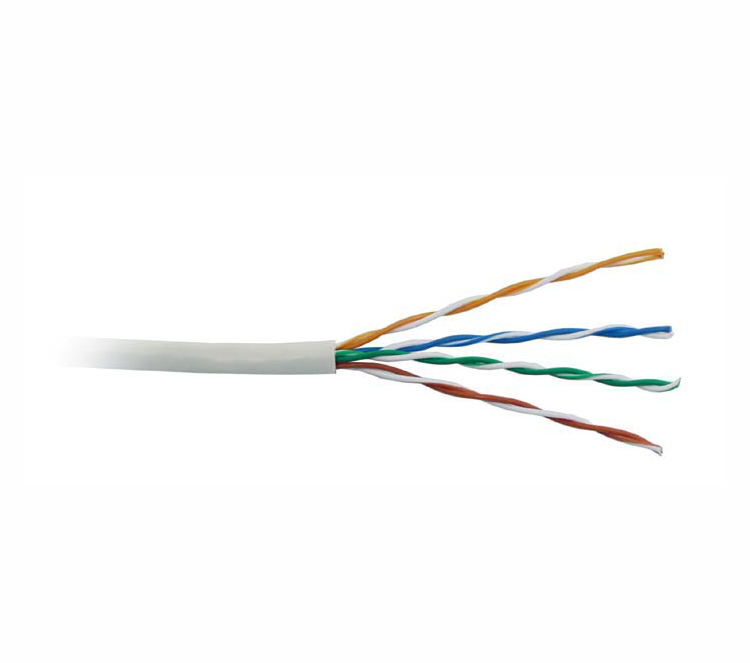
\includegraphics[width=\columnwidth]{./media/image1.jpeg}}

\subsection{Cable Coaxial}
El cable coaxial es otro medio de comunicación de datos ampliamente
usado. Está compuesto por un cable de cobre (conductor interno), rodeado
por un material aislante (llamado ``shell''), que a su vez está envuelto
por un segundo conductor (usualmente una maya de alambres finos) que le
da al cable mayor~protección electromagnética que la del cable de par
trenzados. Finalmente, el cable está cubierto por un material plástico
llamado ``jacket''. El cable coaxial, también llamado coax, es un medio
de alta amplitud de banda que puede llevar miles de señales a la vez.
Este tipo de cable puede transmitir datos a mayor distancia que el cable
de par trenzado y es menos susceptible a la interferencia que el STP. El
cable coaxial permite dos tipos de transmisiones: transmisión de base
ancha (broadband) y transmisión de banda-base (baseband).

\begin{quote}
\noindent\makebox[\textwidth]{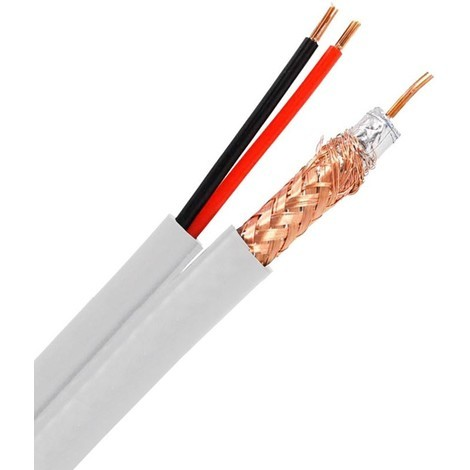
\includegraphics[width=\columnwidth]{./media/image2.jpeg}}
\end{quote}

En la transmisión de base ancha (broadband) un solo cable es dividido
eléctricamente en muchos canales, cada uno llevando diferentes
transmisiones. Esta transmisión es análoga. Utiliza una onda de
transmisión de alta frecuencia, la que se divide en amplitudes de bandas
separadas por los protectores de banda (guardbands) para prevenir
interferencia entre las señales. Usando transmisión de base ancha, una
compañía de televisión por cable puede transmitir múltiples canales a
los hogares individuales mediante un solo cable. Similarmente, el cable
de banda ancha puede transmitir voz, video, datos y otras señales.

~

El otro tipo de transmisión es la banda-base (baseband). En ésta, solo
una señal se transmite a través del cable. Las computadoras utilizan la
transmisión de banda-base para enviar datos a otras computadoras en una
red local. La transmisión de banda-base es digital. El cable y los
conectores usados son menos costosos que los de transmisión de base
ancha.

~

La alta amplitud de banda del cable coaxial lo hace muy atractivo para
una gran variedad de usos. En el pasado, el cable coaxial era usado
principalmente para transmisiones de radio y televisión por cable y para
enlaces entre computadoras y sus equipos auxiliares. Según ha aumentado
la necesidad de líneas de teléfonos adicionales, se ha ido utilizando el
cable coaxial para comunicación~telefónica y de datos.

Sin embargo, el cable coaxial es menos utilizado que el UTP en redes de
área local (LAN), pues el UTP es menos costoso y más fácil de manejar e
instalar. Otra desventaja del cable coaxial es su tamaño, pues es mucho
más grande y pesado que el cable de par trenzado y cable de fibra
óptica.

\subsection{Gu\'ia de Onda}
Una guía de onda es cualquier estructura física que guía ondas
electromagnéticas. El medio dieléctrico en el que esta propagación se
produce está limitado, ya sea por un material conductor (microondas y
radiofrecuencia) o por otro dieléctrico (para frecuencias ópticas).

Dado que la energía se transporta por ondas electromagnéticas, las
características de las guías de onda tales como impedancia, potencia y
atenuación se expresan tales como campos eléctricos y magnéticos
característicos.

Algunos sistemas de telecomunicaciones utilizan la propagación de ondas
en el espacio libre, sin embargo, también se puede transmitir
información mediante el confinamiento de las ondas en cables o guías. En
altas frecuencias las líneas de transmisión y los cables coaxiales
presentan atenuaciones muy elevadas por lo que impiden que la
transmisión de la información sea la adecuada, son imprácticos para
aplicaciones en HF(alta frecuencia) o de bajo consumo de potencia,
especialmente en el caso de las señales cuyas longitudes de onda son del
orden de centímetros, esto es, microondas.

La transmisión de señales por guías de onda reduce la disipación de
energía, es por ello que se utilizan en las frecuencias denominadas de
microondas con el mismo propósito que las líneas de transmisión en
frecuencias más bajas, ya que se presentan poca atenuación para el
manejo de señales de alta frecuencia.

Las paredes conductoras del tubo confinan la onda al interior por
reflexión, debido a la ley de Snell en la superficie, donde el tubo
puede estar vacío o relleno con un dieléctrico. El dieléctrico le da
soporte mecánico al tubo (las paredes pueden ser delgadas), pero reduce
la velocidad de propagación.

\noindent\makebox[\textwidth]{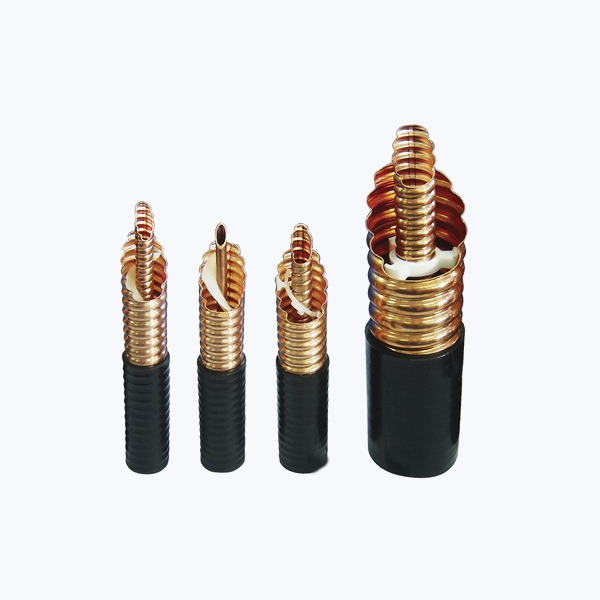
\includegraphics[width=\columnwidth]{./media/image3.jpeg}}

En las guías, los campos eléctricos y los campos magnéticos están
confinados en el espacio que se encuentra en su interior, de este modo
no hay pérdidas de potencia por radiación y las pérdidas en el
dieléctrico son muy bajas debido a que suele ser aire. Este sistema
evita que existan interferencias en el campo por otros objetos, al
contrario de lo que ocurría en los sistemas de transmisión abiertos.

La guía de onda se puede visualizar de manera simplificada en la figura
a continuación, suponiendo que está formada por dos láminas conductoras
y que el transporte de la energía se lleva a cabo mediante reflexiones
continuas y no por medio de corrientes superficiales como en el caso de
las líneas de transmisión.

\noindent\makebox[\textwidth]{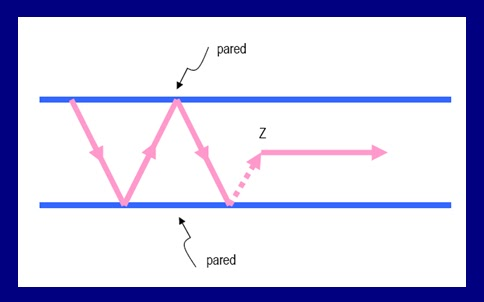
\includegraphics[width=\columnwidth]{./media/image4.jpeg}}

\subsection{Fibra \'Optica}

El cable de fibra utiliza luz para transmitir las señales de datos. La
luz transmite señales digitales usando impulsos de luz para representar
0 y 1. El cable de fibra óptica está compuesto de uno o más cables
pequeños de vidrio o plástico. Cada cable, llamado fibra óptica, es tan
fino como un cabello humano. De hecho, un cable de fibra óptica está
compuesto de muchas fibras ópticas, cada uno rodeada de una barrera de
reflexión~(``cladding''); sobre esta barrera está otra que protege a la
fibra óptica; también se incluye una fibra para fortalecer el cable; y
finalmente una cobertura exterior llamada ``jacket''.

~

La mayor diferencia entre el cable de fibra óptica y el par trenzado o
el cable coaxial es la manera en que las señales de voz y datos se
transmiten. Los cables de cobre transmiten señales eléctricas, mientras
que los cables de fibra óptica transmiten señales por medio de ondas
luminosas (luz). El cable de fibra óptica utiliza un diodo emisor de luz
(LED -- Light-emitting diode) o un láser para enviar pulsos de luz a
través de las fibras. Un LED es una luz de bajo poder creado por un
diodo eléctrico, del mismo tipo de luz usado en algunos relojes
digitales. Un láser provee una fuente de luz más poderosa que el LED,
pero también más costosa. La luz permite que la velocidad de transmisión
de la fibra óptica sea mucho mayor que la del cable de par trenzado o
del cable coaxial.

~

Los cables de fibra óptica están disponibles en tres tipos, que varían
de acuerdo al método usado para transmitir la luz por el cable:

~

\begin{enumerate}
\def\labelenumi{\arabic{enumi}.}
\item
  Fibra multi-modal de índice escalonado (Multimode step index) --
  Utiliza una cobertura plástica o un ``cladding'' parecido a un espejo
  alrededor del cable para reflejar la luz desde el láser o LED. Según
  la luz es reflejada por los lados del cable, se mueve en el cable
  hasta su destino.
\item
  Fibra multi-modal de índice gradual (Multimode graded index) -- En
  este tipo de fibra óptica el núcleo está hecho de varias capas
  concéntricas de material óptico con diferentes índices de refracción.
  El cable varía en densidad, lo que ocasiona curvatura en la luz. Tanto
  el fenómeno de curvatura como el de reflexión causan que la luz se
  mueva hacia el receptor.
\item
  Fibra mono-modal (Single-mode cable) -- Es el tipo de cable más
  rápido. Utiliza un cable muy delgado rodeado por una envoltura que
  concentra el calor. Su principal diferencia es que envía la luz en
  forma directa sin necesidad de reflexión en las paredes de los cables.
\end{enumerate}

Ambos cables de multimodo reflejan la luz a lo largo de la envoltura
mediante el efecto de reflexión (rebote) para transmitir la luz a través
del cable. Es posible que algunos rayos de luz se salgan del patrón de
rebote. Estos rayos viajan mayor distancia y por más tiempo para
alcanzar el final del cable. Esto resulta en pérdida de fortaleza en la
señal (attenuation) y en la dispersión de la señal transmitida.

~

Ventajas del cable de fibra óptica:

\begin{enumerate}
\def\labelenumi{\arabic{enumi}.}
\item
  Alta velocidad de transmisión -- puede transmitir a 100 Mbps, y sigue
  aumentando.
\item
  Seguridad -- Interceptar un cable de cobre es relativamente fácil,
  permitiendo que se pueda robar datos sin que se conozca que está
  ocurriendo. Interceptar un cable de fibra óptica es prácticamente
  imposible, dado su composición. Y si se pudiera, es fácil detectarlo
  por la interrupción de la luz.
\item
  Inmunidad a la interferencia eléctrica
\end{enumerate}

~

Por lo general, la fibra óptica es usada para enlazar redes como LAN,
WAN u otros. Típicamente no se utilizan para enlazar PC individuales a
LAN por el alto costo de las tarjetas de interfase para las PC.
Excepciones a esta regla incluyen ambientes en donde la PC está a más de
100 metros (382 pies) de la conexión de LAN más cercana, ambientes en
donde la interferencia electromagnética es un problema y ambientes en
los cuales es crucial la seguridad.

\noindent\makebox[\textwidth]{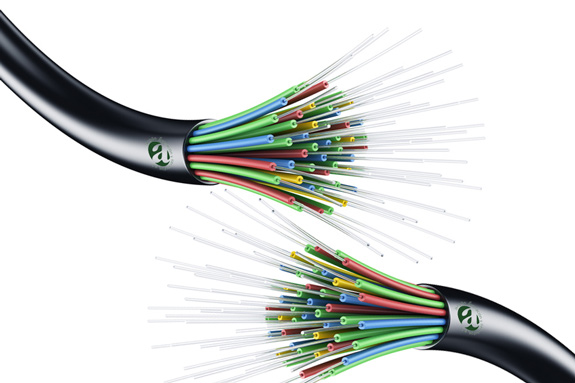
\includegraphics[width=\columnwidth]{./media/image5.jpeg}}

\subsection{LED}

Iluminación led se está convirtiendo en tecnología popular de hoy, y es
utilizada para iluminar hogares, edificios, empresas, negocios, etc. La
tecnología Lifi pretende usar este tipo de iluminación para transmitir
información hacia cualquier dispositivo perceptible a la luz led o que
esté dentro del área de incidencia de esta, mediante cambios de
intensidad de la luz. Por tanto, la tecnología lifi consiste en
transmitir información por medio de la luz led.

Lifi es un tipo de conexión a Internet que usa tecnología que se
caracteriza por transmitir información a través de la luz led que podría
llegar a los 10 Gbps de velocidad. Esto porque la luz se enciende y
apaga hasta 10 mil millones de veces por segundo, lo que hace que se
transforme la información en forma binaria (0 y 1); se aprovecha esta
característica para poder enviar la información a través de la onda de
la luz.

Esta tecnología OWC utiliza la luz de diodos emisores de luz (leds) como
medio de comunicación para redes, móviles, comunicaciones de alta
velocidad, de manera similar a wifi. En el año 2013 se preveía que el
mercado de lifi crecería a una tasa anual compuesta de 82 \% entre 2013
y 2018, para convertirse en un nicho de mercado de más de 6000 millones
de dólares en menos de cuatro años.

Las comunicaciones de luz visible trabajan a modo de parpadeo,
conectando y apagando la corriente a los leds a tal velocidad, que es
imperceptible para el ojo humano. La transmisión de datos a través de
ledes mediante el uso de lifi obligaría a mantener encendidas las
bombillas, pudiéndose atenuar su luminosidad hasta no ser visibles para
el ojo humano y continuaría estando operativa la comunicación. El no
atravesar las ondas de luz las paredes hace que la distancia en las
comunicaciones sean más cortas (pero por sensores se soluciona este
pequeño problema) pero a la misma vez evita muchos problemas de
piratería, al contrario que la comunicación wifi. Tampoco es necesaria
la comunicación en modo línea de visión directa para transmitir la
señal, la luz se refleja en las paredes alcanzando una velocidad de 70
Mbit/s.

\noindent\makebox[\textwidth]{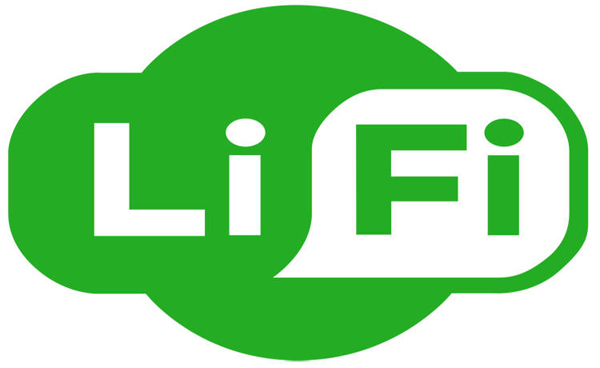
\includegraphics[width=\columnwidth]{./media/image6.jpeg}}

Una de las ventajas de la tecnología lifi es la de poder utilizarse en
zonas sensibles a las áreas electromagnéticas, como puede ser cabinas de
aviones, hospitales y centrales nucleares, sin causar interferencias
electromagnéticas. Ambas conexiones (wifi y lifi) utilizan el espectro
electromagnético para la transmisión de datos, pero mientras que wifi
utiliza ondas de radio, lifi utiliza la luz visible. Según la Comisión
Federal de Comunicaciones (Federal Communications Commission, FCC) de
los Estados Unidos, mientras el espectro electromagnético para el wifi
se está saturando, lifi casi no tiene limitaciones de capacidad. Esto es
debido a que el espectro de luz visible es 10 000 veces más largo que
todo el espectro de radiofrecuencias completo. Las sucesivas
investigaciones indican que se están alcanzando velocidades de
transmisión superior a 10 Gbit/s, mucho más rápida que las primeras
mediciones realizadas desde banda ancha durante el año 2013. Una de sus
principales características es que va a resultar diez veces más barato
que la tecnología wifi.

Algunas de las ventajas que podemos citar son:

\begin{itemize}
\item
  La velocidad de transmisión de datos es muy alta puede ir desde los 15
  Mb/s hasta los 20 Gb/s.
\item
  No existe la interferencia con elementos de radio frecuencia ya que su
  medio de trasmisión es la luz, por lo que se puede usar en lugares
  donde el wifi no llega
\item
  No requiere de circuitos ni antenas o receptores complejos, ya que
  lifi utiliza métodos de modulación parecidos a los infrarrojos
\item
  Al mismo tiempo que se ilumina un lugar se puede tener señal de lifi,
  lo que supondría un ahorro de energía
\item
  Puede permitir conexiones bajo el agua o en aviones, y otros lugares
  donde ahora no se puede tener señal.
\end{itemize}

Aún existen algunas desventajas dentro de las que podemos destacar:

\begin{itemize}
\item
  Las ondas de luz visible no traspasan objetos, como sí lo hacen las
  ondas de radio, por lo que si existe una interferencia se pierde la
  señal
\item
  El alcance del haz de luz de los leds no es muy amplio, pues sólo
  alcanza 5 ó 10 metros.
\end{itemize}

\noindent\makebox[\textwidth]{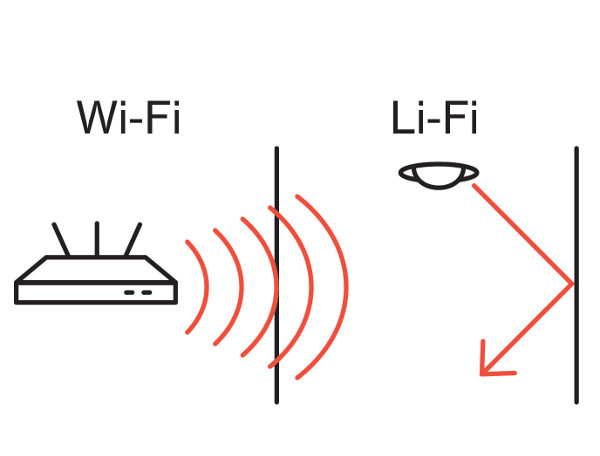
\includegraphics[width=\columnwidth]{./media/image7.jpeg}}

\subsection{LASER}

La transmisión de enormes masas de datos está haciendo llegar a sus
límites la capacidad de la radiofrecuencia, por lo que empresas de todo
el mundo están trabajando en una tecnología láser que pueda servir como
sustituta, una idea que suena a una película de ciencia ficción más que
a la realidad.

La principal ventaja de las emisiones láser es precisamente su mayor
capacidad. Mientras que el récord mundial de la radiofrecuencia es de 36
gigabits por segundo (4,5 GB por segundo), los investigadores del Centro
Aeroespacial de Alemania (DLR, por sus siglas en alemán), ubicado cerca
de Múnich, consiguieron con láser un volumen de 1,7 terabits por segundo
(212,5 GB por segundo).

``En el caso de la radiofrecuencia hay un límite físico, pero la
frecuencia es mucho más elevada en el caso del láser'', explica Wolfram
Peschko, presidente del consejo de administración de Mynaric AG, una
firma surgida del DLR y que está investigando esta técnica para
transformarla en la forma de compartir datos del futuro.

``Partimos de una base muy distinta que las clásicas empresas espaciales
que viven de grandes encargos estatales y fabrican productos
individuales muy costosos'', comenta Peschko, agregando que ``cuando
abordan un proyecto dura años y es realmente caro. Venimos del área
financiada a nivel privado, nuestros tiempos de desarrollo son
relativamente cortos''.

Entre los interesados figuran grandes compañías de alcance mundial como
Facebook, Google y SpaceX, la compañía espacial de Elon Musk, y es que
la cantidad de datos transmitidos a nivel global aumenta constantemente.
``La necesidad actual es de unos 10 gigabits por segundo (1,25 GB por
segundo), pero en un par de años será probablemente de 100 gigabits
(12,5 GB)'', estima Peschko.

\noindent\makebox[\textwidth]{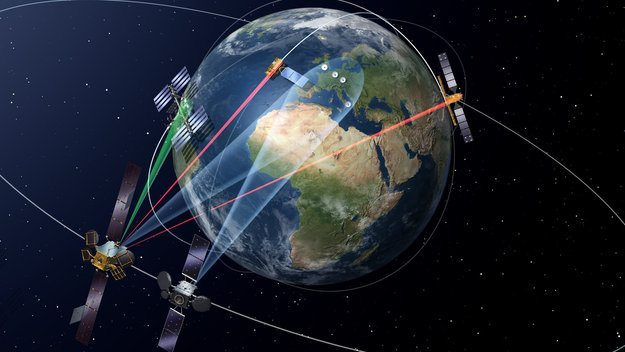
\includegraphics[width=\columnwidth]{./media/image8.jpeg}}

Otro factor es el costo, ya que la comunicación inalámbrica láser es
además mucho más barata que la fibra óptica. ``Si hay que pasar todo
bajo tierra, el proceso es muy caro. Las redes en el aire con ayuda de
nuestra tecnología son hasta 10 veces más baratas que las redes clásicas
que van por el suelo''.

La transmisión óptica es posible en múltiples variantes: desde el
satélite o un avión al suelo o desde un satélite a otro o de un avión a
otro. ``Necesitamos un internet alternativo en el aire'', afirma Markus
Knapek, también del consejo de administración de Mynaric.

\subsection{Microondas}

Además de su aplicación
en \href{https://es.wikipedia.org/wiki/Horno_microondas}{hornos
microondas}, las microondas permiten transmisiones tanto con antenas
terrestres como con satélites. Dada sus frecuencias, del orden de 1 a
10~Ghz, las microondas son muy direccionales y solo se pueden emplear en
situaciones en que existe una línea visual entre emisor y receptor. Los
enlaces de microondas permiten grandes velocidades de transmisión, del
orden de 10 Mbps.

Comunicación vía microondas.~Básicamente un enlace vía microondas
consiste en tres componentes fundamentales: el transmisor, el receptor y
el canal aéreo. El transmisor es el responsable de modular una señal
digital a la frecuencia utilizada para transmitir, el canal aéreo
representa un camino abierto entre el transmisor y el receptor, y como
es de esperarse el receptor es el encargado de capturar la señal
transmitida y llevarla de nuevo a señal digital.

El factor limitante de la propagación de la señal en enlaces microondas
es la distancia que se debe cubrir entre el transmisor y el receptor,
además esta distancia debe ser libre de obstáculos. Otro aspecto que se
debe señalar es que en estos enlaces, el camino entre el receptor y el
transmisor debe tener una altura mínima sobre los obstáculos en la vía,
para compensar este efecto se utilizan torres para ajustar dichas
alturas.

\subsubsection{Algunas de las ventajas}\label{algunas-de-las-ventajas}

\begin{itemize}
\item
  \begin{quote}
  Antenas relativamente pequeñas son efectivas.
  \end{quote}
\item
  \begin{quote}
  A estas frecuencias las ondas de radio se comportan como ondas de luz,
  por ello la señal puede ser enfocada utilizando antenas parabólicas y
  antenas de embudo, además pueden ser reflejadas con reflectores
  pasivos.
  \end{quote}
\item
  \begin{quote}
  Otra ventaja es el ancho de banda, que va de 2 a 24 GHz.
  \end{quote}
\end{itemize}

\subsubsection{Desventajas}\label{desventajas}

Las frecuencias son susceptibles a un fenómeno llamado~Disminución de
Multicamino~(Multipath Fanding), lo que causa profundas disminuciones en
el poder de las señales recibidas.

A estas frecuencias las pérdidas ambientales se transforman en un factor
importante, la absorción de potencia causada por la lluvia puede afectar
dramáticamente el comportamiento del canal.

\subsection{Sat\'elites}

Comunicación por Satélites. Un satélite es transportado a su órbita
abordo de un \href{https://www.ecured.cu/Cohete}{cohete} capaz de
alcanzar la \href{https://www.ecured.cu/Velocidad}{velocidad} suficiente
requerida para no verse influenciado por
el \href{https://www.ecured.cu/index.php?title=Campo_gravitatorio_terrestre\&action=edit\&redlink=1}{campo
gravitatorio terrestre}.

Una vez conseguido esto, es virtualmente posible conseguir cualquier
plano o altitud de la órbita mediante la utilización de modernos
cohetes. El plano de la órbita se denomina inclinación.

Velocidad de la órbita:

Un satélite puede permanecer en su órbita sólo si su velocidad es lo
suficientemente mayor como para vencer
la \href{https://www.ecured.cu/Gravedad}{gravedad} y menor que la
requerida para escapar de la gravedad. La velocidad del satélite es pues
como un compromiso entre esos dos factores, pero ha de ser absolutamente
precisa para la altitud elegida.

$$V={\frac{K}{\sqrt{(r+a)}}}_{\frac{Km}{s}}$$

donde:

V= La velocidad de la órbita en kilómetros por segundo.

a= altitud de la órbita sobre la superficie de la tierra, en Km.

r= el radio medio de la tierra, aproximadamente 6371Km.

K= 630

Aunque la tierra no es perfecta y su radio puede variar, vamos a tomar
que posee un valor de 6371Km.

Periodo de la órbita:

El periodo que posee un satélite viene dado por la siguiente fórmula:

P=K(r+a/r)3/2 minutos~donde P=periodo de una órbita en minutos.
a=altitud de la órbita sobre la superficie terrestre. r=radio medio de
la tierra. K=84.49.

Comunicación por Satélites

En las comunicaciones por satélite, las ondas electromagnéticas se
transmiten gracias a la presencia en el espacio de satélites
artificiales situados en órbita alrededor de la Tierra.

Un satélite actúa básicamente como un repetidor situado en el espacio:
recibe las señales enviadas desde la estación terrestre y las reemite a
otro satélite o de vuelta a los receptores terrestres. En realidad, hay
dos tipos de satélites de comunicaciones:

\begin{itemize}
\item
  Satélites pasivos. Se limitan a reflejar la señal recibida sin llevar
  a cabo ninguna otra tare.
\item
  Satélites activos. Amplifican las señales que reciben antes de
  reemitirlas hacia la Tierra. Son los más habituales y son puestos en
  órbita mediante cohetes espaciales que los sitúan circundando la
  Tierra a distancias relativamente cercanas fuera de la atmósfera.
\end{itemize}

A principios de 1960,
la \href{https://www.ecured.cu/index.php?title=American_Telephone\&action=edit\&redlink=1}{American
Telephone} and~Telegraph Company (AT\&T)~publicó estudios, indicando que
unos cuantos satélites poderosos, de diseño avanzado, podían soportar
más tráfico que toda la red AT\&T de larga distancia. El costo de estos
satélites fue estimado en solo una fracción del costo de las facilidades
de \href{https://www.ecured.cu/index.php?title=Microondas_terrestres\&action=edit\&redlink=1}{microondas
terrestres} equivalentes.

\noindent\makebox[\textwidth]{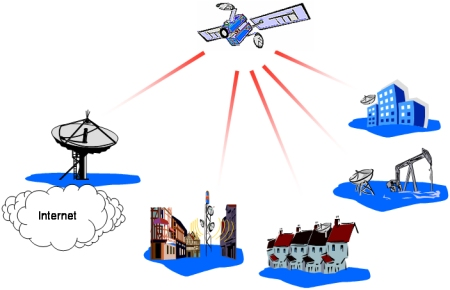
\includegraphics[width=\columnwidth]{./media/image9.jpeg}}

A través de los años, los precios de la mayoría de los bienes y
servicios han aumentado sustancialmente; sin embargo, los servicios de
comunicación, por satélite, se han vuelto mas accesibles cada año. En la
mayoría de los casos, los sistemas de satélites ofrecen mas flexibilidad
que los cables submarinos, cables subterráneos escondidos, radio de
microondas en línea de vista, radio de dispersión troposférica, o
sistemas de \href{https://www.ecured.cu/Fibra_\%C3\%B3ptica}{fibra
óptica}.

Esencialmente, un satélite es
un \href{https://www.ecured.cu/index.php?title=Repetidor_de_radio\&action=edit\&redlink=1}{repetidor
de radio} en el cielo (transponder). Un sistema de satélite consiste de
un transponder, una estación basada en tierra, para controlar el
funcionamiento y una red de usuario, de las estaciones terrestres, que
proporciona las facilidades para transmisión y recepción de tráfico de
comunicaciones, a través del sistema de satélite. Las transmisiones de
satélites se catalogan como bus o carga útil. La de bus incluye
mecanismos de control que apoyan la operación de carga útil. La de carga
útil es la información del usuario que será transportada a través del
sistema. Aunque en los últimos años los nuevos servicios de datos
y \href{https://www.ecured.cu/index.php?title=Radioemisi\%C3\%B3n_de_televisi\%C3\%B3n\&action=edit\&redlink=1}{radioemisión
de televisión} son mas y más demandados, la transmisión de las señales
de teléfono de voz convencional (en forma analógica o digital).

\section{Atenuaci\'on}

La energía de una señal decae con la distancia. La~atenuación~es la
perdida de la potencia de una señal. por ello para que la señal llegue
con la suficiente~energía~es necesario el uso de amplificadores
o~repetidores~~ La~atenuación~se incrementa con la frecuencia, con la
temperatura y con el tiempo.

AFECTA:

La atenuación es la razón principal de que el largo de las redes tenga
varias restricciones. Si la señal se hace muy débil, el equipo receptor
no interceptará bien o no reconocerá esta información. Esto causa
errores, bajo desempeño al tener que transmitir la señal.

\subsection{Bobina de Carga}

La bobina de Pupin o bobina de carga es un inductor que colocado a
intervalos regulares a lo largo de un circuito telefónico formado por
hilos de cobre hace que disminuya la atenuación y la distorsión de
retardo del circuito en la gama de las frecuencias vocales, con el
consiguiente aumento del alcance de la comunicación.

\noindent\makebox[\textwidth]{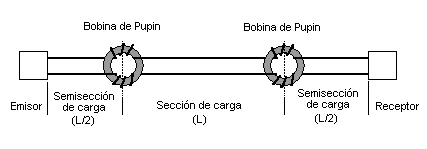
\includegraphics[width=\columnwidth]{./media/image10.png}}

Este, en sus estudios sobre los problemas de transmisión del cable
submarino telegráfico trasatlántico, llegó a determinar la condición que
debía cumplir un medio de transmisión ideal. Esta condición, que se
denominó Condición de Heaviside, en esencia afirma que:

$$R \cdot C = L \cdot G$$

donde R, C, L y G son las constantes primarias del circuito y
representan respectivamente:

R = Resistencia kilométrica en ohmios.

C = Capacidad kilométrica en faradios.

L = Inductancia kilométrica en henrios.

G = Conductancia kilométrica entre hilos del circuito en siemens.

Cuando se cumple la condición de Heaviside la atenuación es mínima e
independiente de la frecuencia, no hay distorsión lineal y el tiempo de
propagación es constante.

En los antiguos circuitos telefónicos de hilo de cobre desnudo de 2 o 3
mm de diámetro, tendidos sobre aisladores, esta condición se cumplía con
cierta aproximación para las frecuencias vocales. El problema surgió con
los cables de pares trenzados, donde R es muy alta al ser los
conductores de menor diámetro, C también es alta al estar muy próximos
entre sí debido al trenzado, en tanto que L es pequeña y G muy pequeña
(el aislamiento entre conductores es muy alto).

Para tratar de cumplir la condición de Heaviside el único parámetro
sobre el que se podía actuar era L.

Para aumentarlo, se apuntaron dos procedimientos:

\begin{itemize}
\item
  El denominado Krarupización ideado por el danés Krarup que consistía
  en rodear los conductores de cobre con otro alambre de material
  magnético con lo que aumenta la inductancia del circuito de forma
  homogénea. Este método era extremadamente caro y solo se usó en
  algunos cables submarinos.
\item
  El otro método es la pupinización consistente en aumentar la
  inductancia, de forma distribuida, mediante la inserción a intervalos
  regulares de bobinas Pupin o de carga.
\end{itemize}

\subsection{Repetidores y Amplificadores}

El repetidor recibe, amplifica y retransmite las señales, con o sin
conversión de frecuencia, procedentes de una estación base (enlace
descendente) y señales procedentes de los equipos móviles en la
dirección opuesta (enlace ascendente) Una ventaja de los repetidores es
que con un equipo podemos dar la extensión de cobertura necesaria de
forma más económica que con un equipo de estación base convencional. Los
repetidores sirven para extender la cobertura de una estación base, pero
no pueden sustituirla, por eso deben estar conectadas siempre a una
estación base. Las aplicaciones típicas de los repetidores son para
hacer llegar la cobertura a túneles, valles e interior de edificios.

En telecomunicaciones, el término repetidor tiene los siguientes
significados normalizados:

\begin{itemize}
  \item Un dispositivo analógico que amplifica una señal de entrada,
  independientemente de su naturaleza (analógica o digital).

  \item Un dispositivo digital que amplifica, conforma, retemporiza o lleva a
  cabo una combinación de cualquiera de estas funciones sobre una señal
  digital de entrada para su retransmisión.
\end{itemize}

Su funcionamiento es el siguiente: toman la señal que circula por una
red y la propagan sin efectuar ningún tipo de traducción o
interpretación de dicha señal. Su efecto sobre el retardo de propagación
de la señal es mínimo.

Dos cables unidos por un repetidor se ven como un mismo cable. Por ello,
sobre ambos debe ir el mismo tipo de red de área local, puesto que los
nodos de ambos segmentos pertenecen a la misma red. Sin embargo, los
cables que unen sí pueden ser diferentes, por ejemplo, coaxial y fibra
óptica.

\noindent\makebox[\textwidth]{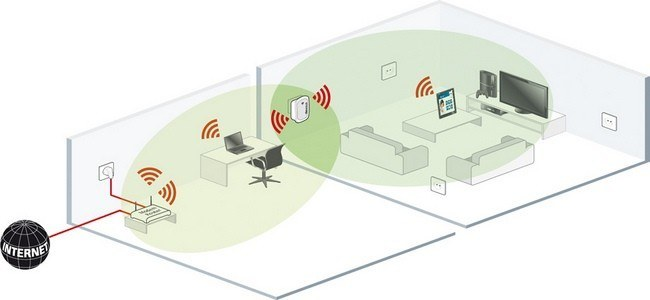
\includegraphics[width=\columnwidth]{./media/image11.jpeg}}

Los diferentes tipos de repetidores que nos podemos encontrar en el
mercado, básicamente se pueden clasificar en los siguientes grandes
grupos:

\begin{itemize}
  \item Repetidores sobre soporte físico

  \item Repetidores sobre enlace inalámbrico    
\end{itemize}

\subsubsection{Repetidores sobre soporte físico}

En este caso la estación base se conecta a través del cable o fibra
correspondiente hasta el repetidor de manera que toda la señal de RF
viaja por el soporte físico, convenientemente adaptada para viajar por
este medio. Las principales ventajas de este tipo de repetidores son la
baja atenuación entre la estación base y el repetidor, el aislamiento
total entre el enlace estación base y repetidor y la comunicación entre
el terminal móvil y el repetidor, además no es necesaria una visión
directa entre la estación base y el repetidor. El principal
inconveniente es el elevado coste de implementación.

Según el medio físico que se utilice en los repetidores sobre soporte
físico pueden ser:

\begin{itemize}
  \item Repetidor sobre cable coaxial

  \item Repetidor sobre cables de pares
  
  \item Repetidor sobre fibra  
\end{itemize}


\subsubsection{Repetidores sobre enlace inalámbrico}

A diferencia de los anteriores no requiere un soporte físico entre la
estación base donante y el repetidor. Existen dos grandes tipos de
repetidores inalámbricos: los repetidores por radio y los repetidores
por infrarrojos.

Las principales ventajas en este tipo de repetidores son: la
implementación sencilla y rápida, y un menor coste de implementación Los
inconvenientes que nos encontramos con estos repetidores son: una mayor
atenuación entre la estación base y el repetidor y la necesidad de que
tengan visión directa.

\subsection{Eco}

Cuando hablamos, el sonido de la voz se transmite de la boca
directamente al aire pero parte de él pasa por el cráneo para llegar a
los oídos. A pesar de que casi no se aprecia, este sonido es fundamental
para escucharse a uno mismo y poder, por tanto, tener un tono de voz
natural. Este sonido es conocido en el mundo de las telecomunicaciones
como tono lateral.

Centrándonos en el eco, las palabras que se vierten a la habitación en
la que se produce la conversación, también rebotan contra las paredes y
de nuevo vuelven a los oídos. Si dicho sonido tarda en volver el
resultado será muy molesto. De hecho, cuanto más retardo haya, más
desagradable es la sensación para el oído humano que es muy sensible a
este fenómeno.\\[2\baselineskip]Existen dos tipos de eco a eliminar. El
eco de línea y el digital. El primero es el conocido como eco de línea,
causado por la diafonía en el cableado o en los convertidores. Un eco
que puede llegar a impedir una comunicación de calidad solamente con el
retorno de menos del 1\% del sonido ya que es un incidente muy molesto.

El segundo tipo de eco es el digital, acústico o espacial. Este puede
darse con frecuencia, con todos los problemas que esto conlleva, ya que
el sonido atraviesa varios convertidores hasta llegar a su destino. Cada
uno de ellos requiere su propio tiempo y esto incrementa el riesgo de
aparición de eco porque al expulsarse más tarde el sonido a la
habitación, se produce una reverberación adicional.

La cancelación de ruido a través de la eliminación de los dos ecos.
Llevándolo a la práctica se consigue mediante un dispositivo que detecta
el eco y crea un sonido de contrafase para anularlo.

\subsection{Optimizar Canal}

Las limitaciones de un canal de transmisión, en cuanto al ancho de
banda, dificultad de transmisión, interferencias, y velocidad surgen
mayormente por las características físicas del canal o transmisor
utilizado.

\subsubsection{Ancho de Banda}

En general, una conexión con ancho de banda alto es aquella que puede
llevar la suficiente información como para sostener la sucesión de
imágenes en una presentación de video.

Tener banda ancha implica usar varios servicios de Internet al mismo
tiempo sin que uno afecte a otro. Podemos chatear, navegar por la Web o
hacer una llamada de VoIP y, al mismo tiempo, descargar un archivo de la
Red sin mayores inconvenientes, ya que la mensajería en general requiere
poco ancho de banda. Hay otros servicios que consumen más ancho de
banda, pero que sin una conexión de este tipo serían impensables.

Todo medio de transmisión disminuye el ancho de banda, razón por la cual
toda señal sufre deformación, para transmitir una señal sin deformación
se requiere un ancho de banda infinito.

\subsubsection{Interferencia}

Se presentan cuando se trabaja con dos señales con bandas de frecuencia
muy próximas.~Son mas relevantes en medio no guiados, sin embargo en los
medios guiados, las emisoras de cables cercanos pueden causar
interferencias por lo que es conveniente apantallar el medio guiado que
se utiliza.

Se puede minimizar esto asegurandose de no permitir que las antenas del
receptor se toquen una con otra al colocar los receptores y asegurarse
que ningún transmisor de radio, incluyendo el transmisor del sistema o
aquellos para otros sistemas inalámbricos, esté aproximadamente entre 10
a 15 pies (3 a 4,5 m) de las antenas receptoras inalámbricas.


\section{An\'alisis de Fourier }

Las ondas armónicas continuas no existen realmente, ya que todos los movimientos ondulatorios están limitados tanto espacial como temporalmente. Utilizando el análisis de Fourier y la transformada de Fourier se pueden describir formas de ondas más complejas como las que producen los instrumentos musicales.

El análisis de Fourier surgió a partir del intento de éste matemático francés por hallar la solución a un problema práctico, la conducción del calor en un anillo de hierro. Demostró que se puede obtener una función discontinua a partir de la suma de funciones continuas. Esta tesis fue defendida por Fourier ante la Academia Francesa, lo que motivó severas objeciones de los matemáticos más importantes de su época como Lagrange, Laplace, etc.

\subsection{Descripci\'on del An\'alisis}

A primera vista, parece que el \href{http://www.sc.ehu.es/sbweb/fisica/ondas/fourier/Fourier.html}{problema de analizar formas de ondas complejas representa una tarea formidable}. Sin embargo, si la forma de la onda es periódica, se puede representar con una precisión arbitraria, mediante la superposición de un número suficientemente grande de ondas senoidales que forman una serie armónica.

Toda función \(f_{(x)}\) periódica de periodo $P$ se puede representar en forma de una suma infinita de funciones armónicas, es decir:

\[g(\xi )={\frac  {1}{{\sqrt  {2\pi }}}}\int _{{-\infty }}^{{+\infty }}f(x)e^{{-i\xi \,x}}dx\]

Es importante notar que la funcion $g(\xi)$ es el resultado de componer todas las funciones arm\'onicas

La transformada de Fourier así definida goza de una serie de \href{https://es.wikipedia.org/wiki/Transformada_de_Fourier}{propiedades de continuidad} que garantizan que puede extenderse a espacios de funciones mayores e incluso a espacios de funciones generalizadas.

Es importante notar que la notacion compleja:
$$z = e^{{-i\xi \,x}} $$
es equivalente a :
$$z = x(\sin({\xi}) - i\cos({\xi}))$$
y por consiguiente, se puede notar , de forma intuitiva su relacion las se\~nales de tipo periodico.

\subsection{Transformada Discreta de Fourier}

la transformada discreta de Fourier o \href{https://es.wikipedia.org/wiki/Transformada_de_Fourier_discreta}{DFT (del inglés, discrete Fourier transform)} es un tipo de transformada discreta utilizada en el análisis de Fourier. Transforma una función matemática en otra, obteniendo una representación en el dominio de la frecuencia, siendo la función original una función en el dominio del tiempo. Pero la DFT requiere que la función de entrada sea una secuencia discreta y de duración finita. Dichas secuencias se suelen generar a partir del muestreo de una función continua, como puede ser la voz humana. Al contrario que la transformada de Fourier en tiempo discreto (DTFT), esta transformación únicamente evalúa suficientes componentes frecuenciales para reconstruir el segmento finito que se analiza. Utilizar la DFT implica que el segmento que se analiza es un único período de una señal periódica que se extiende de forma infinita; si esto no se cumple, se debe utilizar una ventana para reducir los espurios del espectro. Por la misma razón, la DFT inversa (IDFT) no puede reproducir el dominio del tiempo completo, a no ser que la entrada sea periódica indefinidamente. Por estas razones, se dice que la DFT es una transformada de Fourier para análisis de señales de tiempo discreto y dominio finito. Las funciones sinusoidales base que surgen de la descomposición tienen las mismas propiedades.
\\
La entrada de la DFT es una secuencia finita de números reales o complejos, de modo que es ideal para procesar información almacenada en soportes digitales. En particular, la DFT se utiliza comúnmente en procesado digital de señales y otros campos relacionados dedicados a analizar las frecuencias que contiene una señal muestreada, también para resolver ecuaciones diferenciales parciales, y para llevar a cabo operaciones como convoluciones o multiplicaciones de grandes números enteros. Un factor muy importante para este tipo de aplicaciones es que la DFT puede ser calculada de forma eficiente en la práctica utilizando el algoritmo de la transformada rápida de Fourier o FFT (Fast Fourier Transform).

\subsubsection{Transformada Rapida de Fourier (FFT)}

La Transformada rápida de Fourier, conocida por la abreviatura \href{https://es.wikipedia.org/wiki/Transformada_r\%C3\%A1pida_de_Fourier}{FFT} (del inglés Fast Fourier Transform) es un algoritmo eficiente que permite calcular la transformada de Fourier discreta (DFT) y su inversa. La FFT es de gran importancia en una amplia variedad de aplicaciones, desde el tratamiento digital de señales y filtrado digital en general a la resolución de ecuaciones en derivadas parciales o los algoritmos de multiplicación rápida de grandes enteros. Cuando se habla del tratamiento digital de señales, el algoritmo FFT impone algunas limitaciones en la señal y en el espectro resultante ya que la señal muestreada y que se va a transformar debe consistir de un número de muestras igual a una potencia de dos. La mayoría de los analizadores de FFT permiten la transformación de 512, 1024, 2048 o 4096 muestras. El rango de frecuencias cubierto por el análisis FFT depende de la cantidad de muestras recogidas y de la proporción de muestreo.
\\
La transformada rápida de Fourier es de importancia fundamental en el análisis matemático y ha sido objeto de numerosos estudios. La aparición de un algoritmo eficaz para esta operación fue un hito en la historia de la informática.
\\
Sea $x(n)$una señal aperiódica discreta en el tiempo. La transformada discreta de Fourier (DFT, por sus siglas en inglés) de esta señal se define \href{https://engineering.purdue.edu/~ee538/DSP_Text_3rdEdition.pdf}{como}:

\[{\displaystyle X(k)=\sum _{n=0}^{N-1}x(n)e^{-{j2\pi k{\frac {n}{N}}}},\qquad k=0,\dots ,N-1.}\]

en la cual $ X(k) $es un conjunto de números complejos. La evaluación directa de esa fórmula requiere $N^2$ operaciones aritméticas, pero con un algoritmo FFT se puede obtener el mismo resultado con sólo $N\,log \,N$ operaciones. En general, dichos algoritmos dependen de la factorización de \textit{n} pero, al contrario de lo que frecuentemente se cree, existen FFTs para cualquier \textit{n}, incluso con \textit{n} primo.
\\
La idea que permite esta optimización, es la descomposición de la transformada a tratar en otras más simples y éstas a su vez hasta llegar a transformadas de 2 elementos donde k puede tomar los valores 0 y 1. Una vez resueltas las transformadas más simples hay que agruparlas en otras de nivel superior que deben resolverse de nuevo y así sucesivamente hasta llegar al nivel más alto. Al final de este proceso, los resultados obtenidos deben reordenarse.
\\
Dado que la transformada discreta de Fourier inversa es análoga a la transformada discreta de Fourier, con distinto signo en el exponente y un factor 1/''n'', cualquier algoritmo FFT puede ser fácilmente adaptado para el cálculo de la transformada inversa discreta de Fourier (conocida por su sigla inglesa, IDFT). Por lo general, tenemos que:
		
\[{\displaystyle {\begin{aligned}x(n)&={\text{IDFT}}\{X(k)\}\\&={\frac {1}{N}}\sum _{k=0}^{N-1}X(k)e^{j2\pi kn/N}\\&={\frac {1}{N}}\left({\text{DFT}}\left\{{X_{k}}^{*}\right\}\right)^{*}\\\end{aligned}}}\]

donde el símbolo de asterisco (*) denota la conjugada compleja de la expresión que le antecede.

\section{Modulaci\'on}

Engloba el conjunto de técnicas que se usan para transportar información sobre una onda portadora, típicamente una onda sinusoidal. Estas técnicas permiten un mejor aprovechamiento del canal de comunicación lo que posibilita transmitir más información de forma simultánea además de mejorar la resistencia contra posibles ruidos e interferencias. Según la American National Standard for Telecommunications, la modulación es el proceso, o el resultado del proceso, de variar una característica de una onda portadora de acuerdo con una señal que transporta información. El propósito de la modulación es sobreponer señales en las ondas portadoras.
\\
Básicamente, la modulación consiste en hacer que un parámetro de la onda portadora cambie de valor de acuerdo con las variaciones de la señal moduladora, que es la información que queremos transmitir.

\subsection{Se\~nal Portadora}

Una \href{https://es.wikipedia.org/wiki/Onda_portadora}{señal portadora es una onda eléctrica} que puede ser modificada en alguno de sus parámetros por la señal de información (sonido, imagen o datos) para obtener una señal modulada y que se transporta por el canal de comunicaciones.
\\
El uso de una onda portadora también soluciona muchos problemas de circuito, antena, propagación y ruido. Por ello, una antena práctica debe tener un tamaño aproximado al de la longitud de onda de la onda electromagnética de la señal que se va a transmitir. Si las ondas de sonido se difundieran directamente en forma de señales electromagnéticas , la antena tendría que tener más de un kilómetro de altura. Usando frecuencias mucho más altas para la portadora, el tamaño de la antena se reduce significativamente porque las frecuencias más altas tienen longitudes de ondas más cortas.
\\
Una emisora de radio AM normalmente tiene una serie de letras asociadas: por ejemplo, KPBS. Sin embargo, una forma más práctica de referirse a una emisora de radio es por su frecuencia portadora, como 101.1 MHZ, que es la frecuencia con la que se debe sintonizar la radio. En el caso de las FM, la frecuencia portadora es de 87 a 108 MHZ. El uso de frecuencias portadoras en las FM ha añadido complejidad en cuanto que la frecuencia portadora cambia con el salto de frecuencia o la secuencia de chipping directa para que la señal sea más inmune a la interferencia y el ruido. El chipping es el proceso consistente en convertir cada bit de datos en una cadena de chips expandida denominada secuencia de chipping. Es el mecanismo que permite a los dispositivos inalámbricos leer datos cuando se pierden porciones de señal
\\
El proceso de recuperar la información de las ondas portadoras se denomina demodulación. En esencia, es invertir los pasos utilizados para modular los datos. En general, a medida que los esquemas de transmisión o modulación(compresión) se hacen más complejos y la velocidad de transmisión de datos aumenta, la inmunidad al ruido se reduce y la cobertura disminuye.
 
\subsection{Tipos de Modulaci\'on}

Las formas básicas de Modulación son:

\begin{itemize}
	\item Amplitud
	\begin{itemize}
		\item Modulación en Amplitud - Doble banda lateral con portadora - AM
		\item Doble banda lateral sin portadora - DBL-SP
		\item Banda lateral única - BLU
	\end{itemize}
	\item Angular
	\begin{itemize}
		\item Modulación en Frecuencia - FM
		\item Modulación en Fase - PM
	\end{itemize}
\end{itemize}

\subsubsection{Modulación Analógica}

Las tres técnicas de modulación analógica son:
\begin{itemize}
	\item Modulación de la amplitud (AM o amplitud modulada).
	\item Modulación de la frecuencia (FM o frecuencia modulada).
	\item Modulación de la fase (PM o fase modulada).
\end{itemize}


La mayoría de los sistemas de comunicación utilizan alguna de estas tres técnicas de modulación básicas, o una combinación de ellas. Las Radios están basadas en AM y FM siendo la FM la de mejor calidad debido a la ventaja que tiene por manejar mayores frecuencias y mayores anchos de banda que mejoran la percepción por el contenido que se puede transmitir.

\subsubsection{Modulación Digital}

Los siguientes son algunos de casos extremos de estas técnicas:

\begin{itemize}
		\item Modulación por desplazamiento de amplitud (ASK, Amplitude Shift Keying)
		Desactiva la amplitud durante toda la trayectoria
		
		\item Modulación por desplazamiento de frecuencia (FSK,Frecuency Shift Keying
		Salta a una frecuencia extrema.
		
		\item Modulación por desplazamiento de fase (PSK, Phase Shift Keying)
		Desplaza la fase 180 grados.
\end{itemize}

\noindent\makebox[\textwidth]{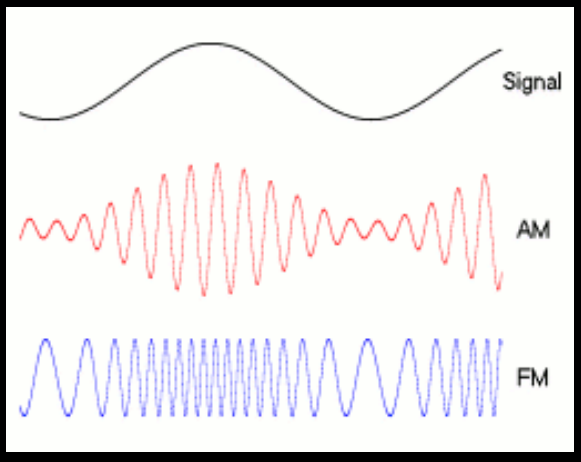
\includegraphics[width=\columnwidth]{./media/image12.png}}

\subsection{Tecnicas de modulación}

Dependiendo del parámetro sobre el que se actúe, tenemos los distintos tipos de modulación:

\begin{itemize}
	\item Modulación en doble banda lateral (DSB)
	\item Modulación de amplitud (AM)
	\item Modulación de fase (PM)
	\item Modulación de frecuencia (FM)
	\item Modulación banda lateral única (SSB, ó BLU)
	\item Modulación de banda lateral vestigial (VSB, VSB-AM, ó BLV)
	\item Modulación de amplitud en cuadratura (QAM)
	\item Modulación por división ortogonal de frecuencia (OFDM), también conocida como 'Modulación por multitono discreto' (DMT)
	\item Modulación de Espectro ensanchado por secuencia directa (DSSS)
	\item Modulación por longitud de onda
	\item Modulación en anillo
\end{itemize}

Cuando la OFDM se usa en conjunción con técnicas de codificación de canal, se denomina Modulación por división ortogonal de frecuencia codificada (COFDM).

También se emplean técnicas de modulación por impulsos, pudiendo citar entre ellas:

\begin{itemize}
	\item Modulación por impulsos codificados (PCM)
	\item Modulación por anchura de pulsos (PWM)
	\item Modulación por duración de pulsos (PDM)
	\item Modulación por amplitud de pulsos (PAM)
	\item Modulación por posición de pulsos (PPM)
\end{itemize}


Cuando la señal es una indicación simple on-off a baja velocidad, como una transmisión en código Morse o radioteletipo (RTTY), la modulación se denomina manipulación, modulación por desplazamiento, así tenemos:

\begin{itemize}
	\item Modulación por desplazamiento de amplitud (ASK)
	\item Modulación por desplazamiento de frecuencia (FSK)
	\item Modulación por desplazamiento de fase (PSK)
	\item Modulación por desplazamiento de amplitud y fase (APSK o APK)	
\end{itemize}




La transmisión de radioteletipo (RTTY) puede ser considerada como una forma simple de Modulación por impulsos codificados
\\
Cuando se usa el código Morse para conmutar on-off la onda portadora, no se usa el término 'manipulación de amplitud', sino operación en onda continua (CW).
\\
La modulación se usa frecuentemente en conjunción con varios métodos de acceso de canal. Otras formas de modulación más complejas son (PSK),(QAM),(I/Q),(QFSK),etc. 

\section{Amplitud modulada}

La modulación de amplitud o amplitud modulada (AM) es una técnica utilizada en la comunicación electrónica, más comúnmente para la transmisión de información a través de una onda transversal de televisión. La modulación en amplitud (AM) funciona mediante la variación de la amplitud de la señal transmitida en relación con la información que se envía. Contrastando esta con la modulación de frecuencia, en la que se varía la frecuencia, y la modulación de fase, en la que se varía la fase. A mediados de la década de 1870, una forma de modulación de amplitud, inicialmente llamada "corrientes ondulatorias", fue el primer método para enviar con éxito audio a través de líneas telefónicas con una calidad aceptable. 

\subsection{Demodulaci\'on}

Existen dos posibilidades para la demodulación de una señal $f(t)$ modulada en AM. La primera de ellas, la más simple, es sólo posible en caso de que se cumpla la condición siguiente:

\[\big\| f_n(t) \big\| \leq m \]

En este supuesto, la envolvente de la señal modulada, esto es $1 + m \cdot f_n(t)$ es siempre positiva y para recuperar la señal moduladora es suficiente con un receptor que capte dicha envolvente. Esto se consigue con un simple circuito rectificador con carga capacitiva. Así funcionaba la pionera radio de galena.

La otra opción para la demodulación de la señal modulada en AM es utilizar el mismo tipo de demodulación que se usa en las otras modulaciones lineales. Se trata del demodulador coherente. Para ello, es necesario conocer la frecuencia de la portadora \textit{}{$w_p$} y, en ocasiones, también la fase, lo que requiere la utilización de un PLL (''Phase Lock Loop''). En este otro supuesto, no es necesario que el índice de modulación sea menor que la unidad, o lo que es lo mismo, no es necesario que la envolvente [1 + m·x(t)] sea siempre positiva.

El demodulador coherente utiliza la siguiente propiedad matemática de la función coseno:

\[\cos^2(\phi) = \frac {1}{2} + \frac {\cos(2\phi)}{2}\]

para multiplicar la función $S(t)$ por la portadora:

\[S_D(t) = S(t) \cos(w_c)= \frac{1 + m \cdot f_n(t)}{2} + \frac{\cos(2w_c)}{2}\]

A partir de esto, con un filtro paso bajo y un supresor de continua, se obtiene la señal $f(t)$.

\subsection{Índice de modulación}

El índice de modulación de AM es una medida de la variación de amplitud que rodea una portadora no modulada. Al igual que con otros índices de modulación, en AM esta cantidad (también llamada "profundidad de modulación") indica la variación introducida por la modulación respecto al nivel de la señal original. En AM, se refiere a las variaciones en la amplitud de la portadora y se define como: 
$$h = \frac{\mathrm{valor\ m\acute{a}ximo\  de\ } m(t)}{A} = \frac{M}{A}$$ donde $M$ y $A$ son la amplitud del mensaje y la amplitud de la portadora, respectivamente.

Así que si $h=0,5$, la amplitud de la portadora varía en un 50\% por encima (y por debajo) de su nivel original; para $h=1,0$, la señal varía en un 100\%. Para evitar la distorsión, la profundidad de modulación no deberá exceder del 100\%. En sistemas de transmisión por lo general se incorporará un circuito limitador para asegurar cumplir este requisito. Sin embargo, los demoduladores de AM pueden ser diseñados para detectar la inversión de fase que se produce cuando la modulación excede el 100\%, y automáticamente corrige este defecto. A continuación se muestran unas imágenes en las que se pueden observar los resultados de modular con diferentes índices de modulación.
\\
\\
\noindent\makebox[\textwidth]{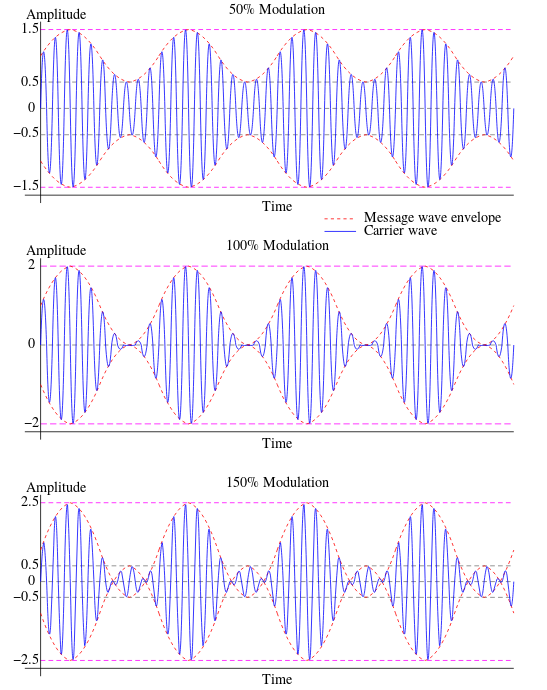
\includegraphics[width=0.9\columnwidth]{./media/image13.png}}

\section{Frecuencia Modulada}

La modulación de frecuencia o frecuencia modulada (FM) es una técnica de modulación que permite transmitir información a través de una onda portadora variando su frecuencia.
En aplicaciones analógicas, la frecuencia instantánea de la señal modulada es proporcional al valor instantáneo de la señal moduladora.
Se puede enviar datos digitales por el desplazamiento de la onda de frecuencia entre un conjunto de valores discretos, modulación conocida como modulación por desplazamiento de frecuencia.
\\
La modulación de frecuencia se usa comúnmente en las radiofrecuencias de muy alta frecuencia por la alta fidelidad de la radiodifusión de la música y el habla. El sonido de la televisión analógica también se difunde por medio de FM. Se utiliza un formulario de banda estrecha para comunicaciones de voz en la radio comercial y en las configuraciones de aficionados. El tipo que se usa en la radiodifusión FM generalmente se llama amplia-FM o W-FM (de la siglas en inglés "Wide-FM"). En la radio de dos vías, se utiliza la banda estrecha o N-FM (de la siglas en inglés "Narrow-FM") para ahorrar ancho de banda. Además, se utiliza para enviar señales al espacio.
\\
La modulación de frecuencia también se utiliza en las frecuencias intermedias de la mayoría de los sistemas de vídeo analógico, incluyendo VHS, para registrar la luminancia (blanco y negro) de la señal de video. La modulación de frecuencia es el único método factible para la grabación de video y para reproducir la cinta magnética sin la distorsión extrema, como las señales de vídeo con una gran variedad de componentes de frecuencia, de unos pocos hercios a varios megahercios; también es demasiado amplia para trabajar con equalisers con la deuda al ruido electrónico debajo de -60 dB. La FM también mantiene la cinta en el nivel de saturación, y, por tanto, actúa como una forma de reducción de ruido del audio, y un simple corrector puede enmascarar variaciones en la salida de la reproducción, y la captura del efecto de FM elimina a través de impresión y pre-eco. Un piloto de tono continuo, si se añade a la señal (se hizo en V2000 o video 2000 y muchos formatos de alta banda) puede mantener el temblor mecánico bajo control y ayudar al tiempo de corrección.
\\
Dentro de los avances más importantes que se presentan en las comunicaciones, uno de los más importantes es, sin duda, la mejora de un sistema de transmisión y recepción en características como la relación señal-ruido, pues permite una mayor seguridad en las mismas. Es así como el paso de modulación de amplitud (AM), a la modulación de frecuencia (FM) establece un importante avance no solo en el mejoramiento que presenta la relación señal ruido, sino también en la mayor resistencia al efecto del desvanecimiento y a la interferencia, tan comunes en AM.
Esta demostración de General Electric en 1940 comprobó la resistencia de la señal de modulación de frecuencia a las interferencias. Cerca del prototipo de receptor de radio (en el centro) se realiza una descarga eléctrica de un millón de voltios. Durante la sintonía en AM, el grado de interferencia fue tal que sólo logró escucharse el resultado de la descarga eléctrica. Cuando se cambió al modo FM, la música logró escucharse con sólo una pequeña cantidad de estática.
\\
La modulación de frecuencia también se utiliza en las frecuencias de audio para sintetizar sonido. Está técnica, conocida como síntesis FM, fue popularizada a principios de los sintetizadores digitales y se convirtió en una característica estándar para varias generaciones de tarjetas de sonido de computadoras personales. 
\\
\\
\noindent\makebox[\textwidth]{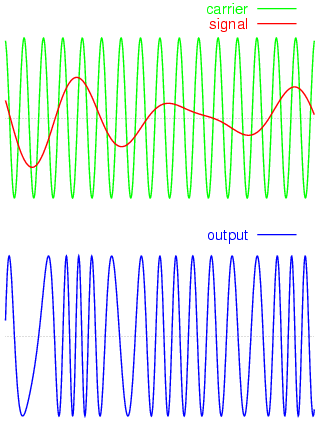
\includegraphics[width=\columnwidth]{./media/image14.png}}

\subsection{Funcionamiento}

\subsubsection{Modulador de FM}

La modulación de una portadora sobre FM, aunque se puede realizar de varias formas, resulta un problema delicado debido a que se necesitan dos características contrapuestas: estabilidad de frecuencia y que la señal moduladora varíe la frecuencia. Por ello, la solución simple de aplicar la señal moduladora a un oscilador controlado por tensión (VCO) no es satisfactoria.
\begin{itemize}
	\item \textbf{Modulación del oscilador}. En oscilador estable, controlado con un cristal piezoeléctrico, se añade un condensador variable con la señal moduladora (varactor). Eso varía ligeramente la frecuencia del oscilador en función de la señal moduladora. Como la excursión de frecuencia que se consigue no suele ser suficiente, se lleva la señal de salida del oscilador a multiplicadores de frecuencia para alcanzar la frecuencia de radiodifusión elegida.
	\item \textbf{Moduladores de fase}. Un modulador de FM se puede modelar exactamente como un modulador de PM con un integrador a la entrada de la señal moduladora.
	\item \textbf{Modulador con PLL}. Vuelve a ser el VCO, pero ahora su salida se compara con una frecuencia de referencia para obtener una señal de error, de modo que se tiene una realimentación negativa que minimiza dicho error. La señal de error se filtra para que sea insensible a las variaciones dentro del ancho de banda de la señal moduladora, puesto que estas variaciones son las que modulan la salida del VCO. Este método se ha impuesto con la llegada de los PLL integrados ya que ha pasado de ser el más complejo y costoso a ser muy económico. Presenta otras ventajas, como es poder cambiar de frecuencia para pasar de un canal a otro y mantiene coherentes todas las frecuencias del sistema.
\end{itemize}

\subsubsection{Demodulador de FM}

También es más complejo que el de AM. Se utilizan sobre todo dos métodos:

\begin{itemize}
	\item \textbf{Discriminador reactivo}. Se basa en llevar la señal de FM a una reactancia, normalmente bobinas acopladas, de forma que su impedancia varíe con la frecuencia. La señal de salida aparece, entonces, modulada en amplitud y se detecta con un detector de envolvente. Existían válvulas específicas para esta tarea, consistentes en un doble-diodo-triodo. Los dos diodos forman el detector de envolvente y el triodo amplifica la señal, mejorando la relación señal/ruido.
	
	\item \textbf{Detector con PLL (Phase Locked Loop)}. La señal del PLL proporciona la señal demodulada. Existen muchas variaciones según la aplicación, pero estos detectores suelen estar en circuitos integrados que, además, contienen los amplificadores de RF y frecuencia intermedia. Algunos son una radio de FM completa (TDA7000).
\end{itemize}

\subsection{Expresi\'on Anal\'itica}

\[y_{fm}(t)=A_{c}\cos[w_ct + 2 \pi f_D \int_0^t X_{N}{(\alpha)} d\alpha]\]

Donde:

\begin{itemize}
	\item $X_{N}$ es la señal mensaje (moduladora) normalizada.

	\item $f_D$ es la máxima desviación en frecuencia, máximo valor que toma la desviación instantánea de frecuencia.

	\item $A_{c}$ es la amplitud de la señal.
\end{itemize}

\section{Modulación de fase}

Es una modulación que se caracteriza porque la fase de la onda portadora varía en forma directamente proporcional de acuerdo con la señal moduladora. La modulación de fase no suele ser muy utilizada porque se requieren equipos de recepción más complejos que los de frecuencia modulada. Además puede presentar problemas de ambigüedad para determinar si una señal tiene una fase de 0º o 180º.
\\
\\
\noindent\makebox[\textwidth]{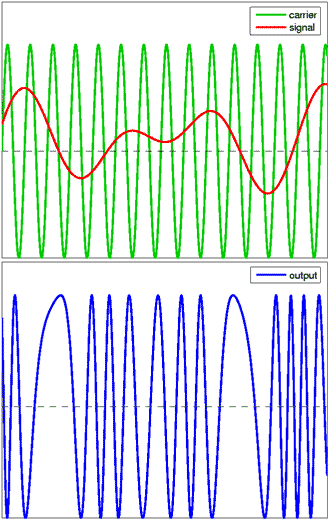
\includegraphics[width=0.9\columnwidth]{./media/image15.png}}

\subsection{Teoría}

Supongamos que la señal a ser transmitida o moduladora es $\scriptstyle m(t)$ y que la señal portadora se expresa como:

\[c(t) = A_c\sin\left(\omega_\mathrm{c}t + \phi_\mathrm{c}\right).\]

Donde:
\begin{itemize}
	\item $\scriptstyle \omega_\mathrm{c}$ = Frecuencia angular de la portadora.
\end{itemize}

La señal resultante es descrita por la siguiente ecuación:

\[y(t) = A_c\sin\left(\omega_\mathrm{c}t + m(t) + \phi_\mathrm{c}\right).\]

Esto demuestra como $\scriptstyle m(t)$ modula la fase; mientras mayor sea el valor de la señal en determinado punto en el tiempo, mayor será el desfase de la onda portadora en ese punto. Esto también puede ser visto como un cambio en la frecuencia de la onda portadora y así la Modulación de Fase se puede considerar como un caso especial de la \textbf{FM} en la cual la modulación en frecuencia es dada por la derivada respecto al tiempo de la modulación de fase.

Las matemática del comportamiento de la densidad espectral revela que existen dos regiones de interés particular: 

\begin{itemize}
	\item Para señales de amplitud pequeña, la modulación de fase es similar a la amplitud modulada AM y muestra, por tanto, el "doblado" de su ancho de banda base y pobre eficiencia.

	\item Para señales senoidales grandes, esta modulación es similar a la FM, y su ancho de banda es aproximadamente:
\end{itemize}

\[2\left(h + 1\right)f_\mathrm{M}\]

dond $\textstyle f_\mathrm{M} = \omega_\mathrm{m}/2\pi$ y $\textstyle h$ es el índice de modulación. Esto también se conoce como la \textbf{Regla de Carson} para la modulación de fase. El índice de modulación, en este caso, indica cuanto varía la fase alrededor del valor sin modulación en la onda portadora:

\[h= \Delta \theta\]

Donde $\scriptstyle \Delta \theta$ es la desviación pico en fase.


\end{document}
